\section{BigchainDB Description}\label{sec:bigchaindb}

\subsection{Principles}
Rather than trying to scale up blockchain technology, BigchainDB starts with a “big data” distributed database, and adds blockchain characteristics.
It avoids the technology choices that plague Bitcoin, such as full replication and broadcast communication.

We built BigchainDB on top of an enterprise-grade distributed DB, from which BigchainDB inherits high throughput, high capacity, a full-featured NoSQL query language, efficient querying, and permissioning. Nodes can be added to increase throughput and capacity.

Since the big data DB has its own built-in consensus algorithm to tolerate benign faults, we exploit that solution directly.
We “get out of the way” of the algorithm to let it decide which transactions to write, and what the block order is.
We disallow private, peer-to-peer communication between the nodes except via the DB’s built-in communication, for great savings in complexity and for reduced security risk\footnote{Though we must vigilantly exercise restraint in design, as intuition is to just get the nodes talking directly!}.
This means that malicious nodes cannot transmit one message to part of the network and different message to other part of the network. Everytime a node ``speaks'' all the others can listen.

\subsection{High-Level Description}
We focused on the adding the following blockchain features to the DB:
\begin{enumerate}
 \item \textbf{Decentralized control}, where “no one” owns or controls a network;
 \item \textbf{Immutability}, where written data is tamper-resistant (“forever”); and
 \item \textbf{The ability to create \& transfer assets} on the network, without reliance on a central entity.
\end{enumerate}

Decentralized control is achieved via a DNS-like federation of nodes with voting permissions.
Other nodes can connect to read, and propose transactions; this makes it a super-peer P2P network \cite{ozsu2011principles}.
The voting operates at a layer above the DB’s built in consensus.
Quorum is a majority of votes.
For speed, all transactions are written independent of their validity; votes are done a posteriori.
A network with $2f+1$ voting nodes that communicate openly (ie. through the database) can tolerate $f$ malicious nodes\footnote{It is $2f+1$ and not $3f+1$ because digital signatures are employed. Section \ref{subsec:distributed:paxos} has details.} \cite{lamport1982byzantine}.

Immutability is via an ordered sequence of blocks where each block holds an ordered sequence of transactions; and a block’s hash is over its transactions and related data; that is, a block chain.
Blocks are written, then voted upon.
Chainification actually happens at voting time.
A block doesn't have a top-level link to the previous block.
Instead, it has a list of votes, and each vote has a “previous block” attribute pointing to the id of the block coming before it.

Any entity with asset-issuance permissions can issue an asset; any entity with asset-transfer permissions and the asset’s private key may transfer the asset.
This means hackers or compromised system admins cannot arbitrarily change data, and there is no single-point-of-failure risk.

\subsection{Architecture}
Figure \ref{fig:bigchaindb_architecture} illustrates the architecture of the BigchainDB system.
The BigchainDB system presents its API to clients as if it was a single blockchain database.
Under the hood, there are actually two distributed databases\footnote{This can be implemented as two databases, or as two tables in the same database. While there is no practical difference, for the sake of clarity we describe it as two separate databases.}, $\mathbf{S}$ (transaction set or “backlog”) and $\mathbf{C}$ (block chain), connected by the BigchainDB Consensus Algorithm (BCA).
The BCA runs on each signing node.
Non-signing clients may connect to BigchainDB; depending on permissions they may be able to read, issue assets, transfer assets, and more; section \ref{sec:permissioning} explores this more.

\begin{figure}[!ht]
  \centering
  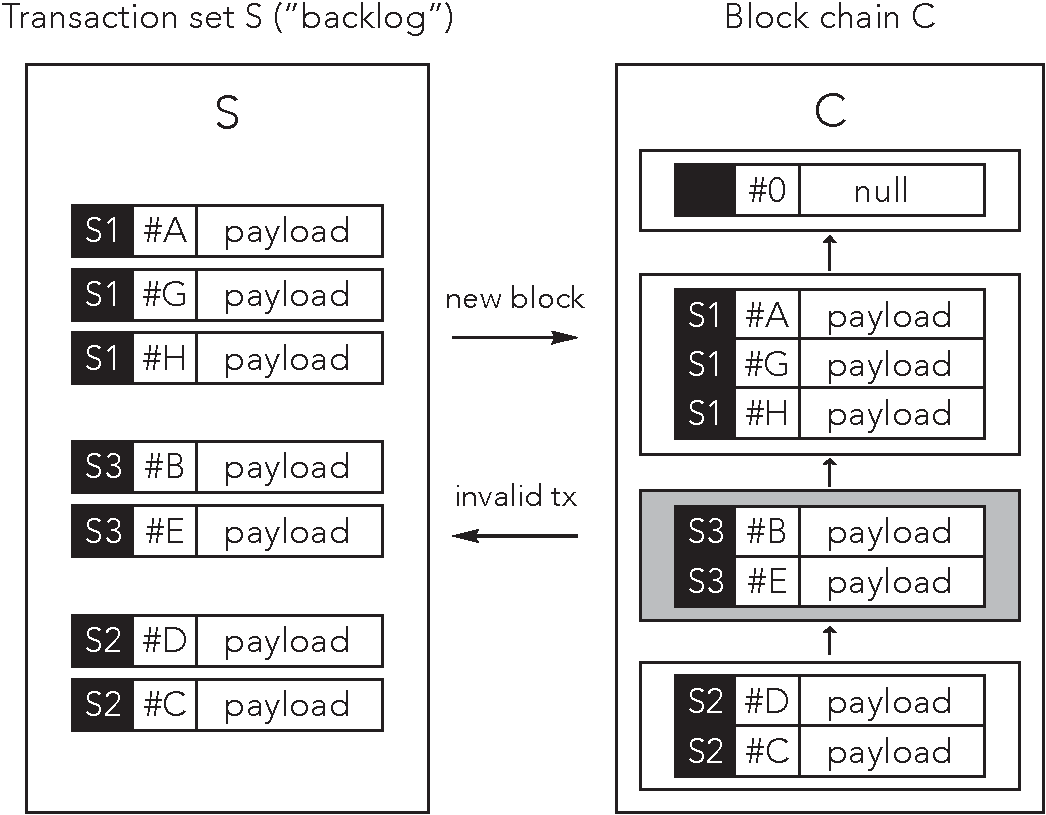
\includegraphics[width=0.7\textwidth]{figure_3.pdf}
  \caption{Architecture of BigchainDB system.
  There are two big data distributed databases: a Transaction Set $\mathbf{S}$ (left) to take in and assign incoming transactions, and a Blockchain $\mathbf{C}$ (right) holding ordered transactions that are “etched into stone”.
  The signing nodes running the BigchainDB Consensus Algorithm update $\mathbf{S}$, $\mathbf{C}$, and the transactions (txs) between them.}
  \label{fig:bigchaindb_architecture}
\end{figure}

Each of the distributed DBs, $\mathbf{S}$ and $\mathbf{C}$, is an off-the-shelf big data DB.
We do not interfere with the internal workings of each DB; in this way, we get to leverage the scalability properties of the DBs, in addition to features like revision control and benefits like battle-tested code.
Each DB may hold any number of transactions.
Each may be implemented in hardware in any number of hard drives or flash drives.
Each is running its own internal Paxos-like consensus algorithm for consistency among the drives.

The first DB holds the “backlog” transactions—an unordered set of transactions $\mathbf{S}$.
When a transaction comes in, it is assigned to a single signing node to process.
There are $N$ signing nodes. $\mathbf{S}_k = \{\mathbf{t}_{k,1}, \mathbf{t}_{k,2}, \dots\}$ is the set of transactions assigned to node $\mathbf{k}$.

Node $\mathbf{k}$ running the BigchainDB Consensus Algorithm (BCA) processes transactions from $\mathbf{S}$ as follows: It moves transactions from the unordered set $\mathbf{S}_k$ into an ordered list, creates a block for the transactions, and puts the block into the second database $\mathbf{C}$.
$\mathbf{C}$ is an ordered list of blocks where each block has reference to a parent block and its data, that is, a blockchain.

A signing node can vote on whether it considers a block \textsf{\textit{valid}} or \textsf{\textit{invalid}}. To decide, the signing node checks the validity of every transaction in the block, and if it finds an invalid transaction, then the signing node votes that the block is \textsf{\textit{invalid}}.
If the signing node finds no invalid transactions, then it votes that the block is \textsf{\textit{valid}}.

Each block starts out as \textsf{\textit{undecided}}, with no votes from signing nodes.
Once there is majority of positive (\textsf{\textit{valid}}) votes for a block, or a majority of negative (\textsf{\textit{invalid}}) votes, the block goes from \textsf{\textit{undecided}} to \textsf{\textit{decided\_valid}} or \textsf{\textit{decided\_invalid}}, respectively, and voting on the block stops.
Once it is decided, it can be treated as “etched into stone.” This process is similar to the idea of multiple confirmations in Bitcoin blockchain.

A block $\mathbf{B}$ in the blockchain has an ID, timestamp, the actual transactions, and vote information. Section \ref{subsec:bigchaindb:models} describes block, transaction, and voting models precisely.

\subsection{Behavioral Description}
This section examines the flow of transactions from a client to a given server node.
Each server node has its own view of the transaction backlog $\mathbf{S}$, and the chain $\mathbf{C}$.

\begin{figure}[!ht]
  \centering
  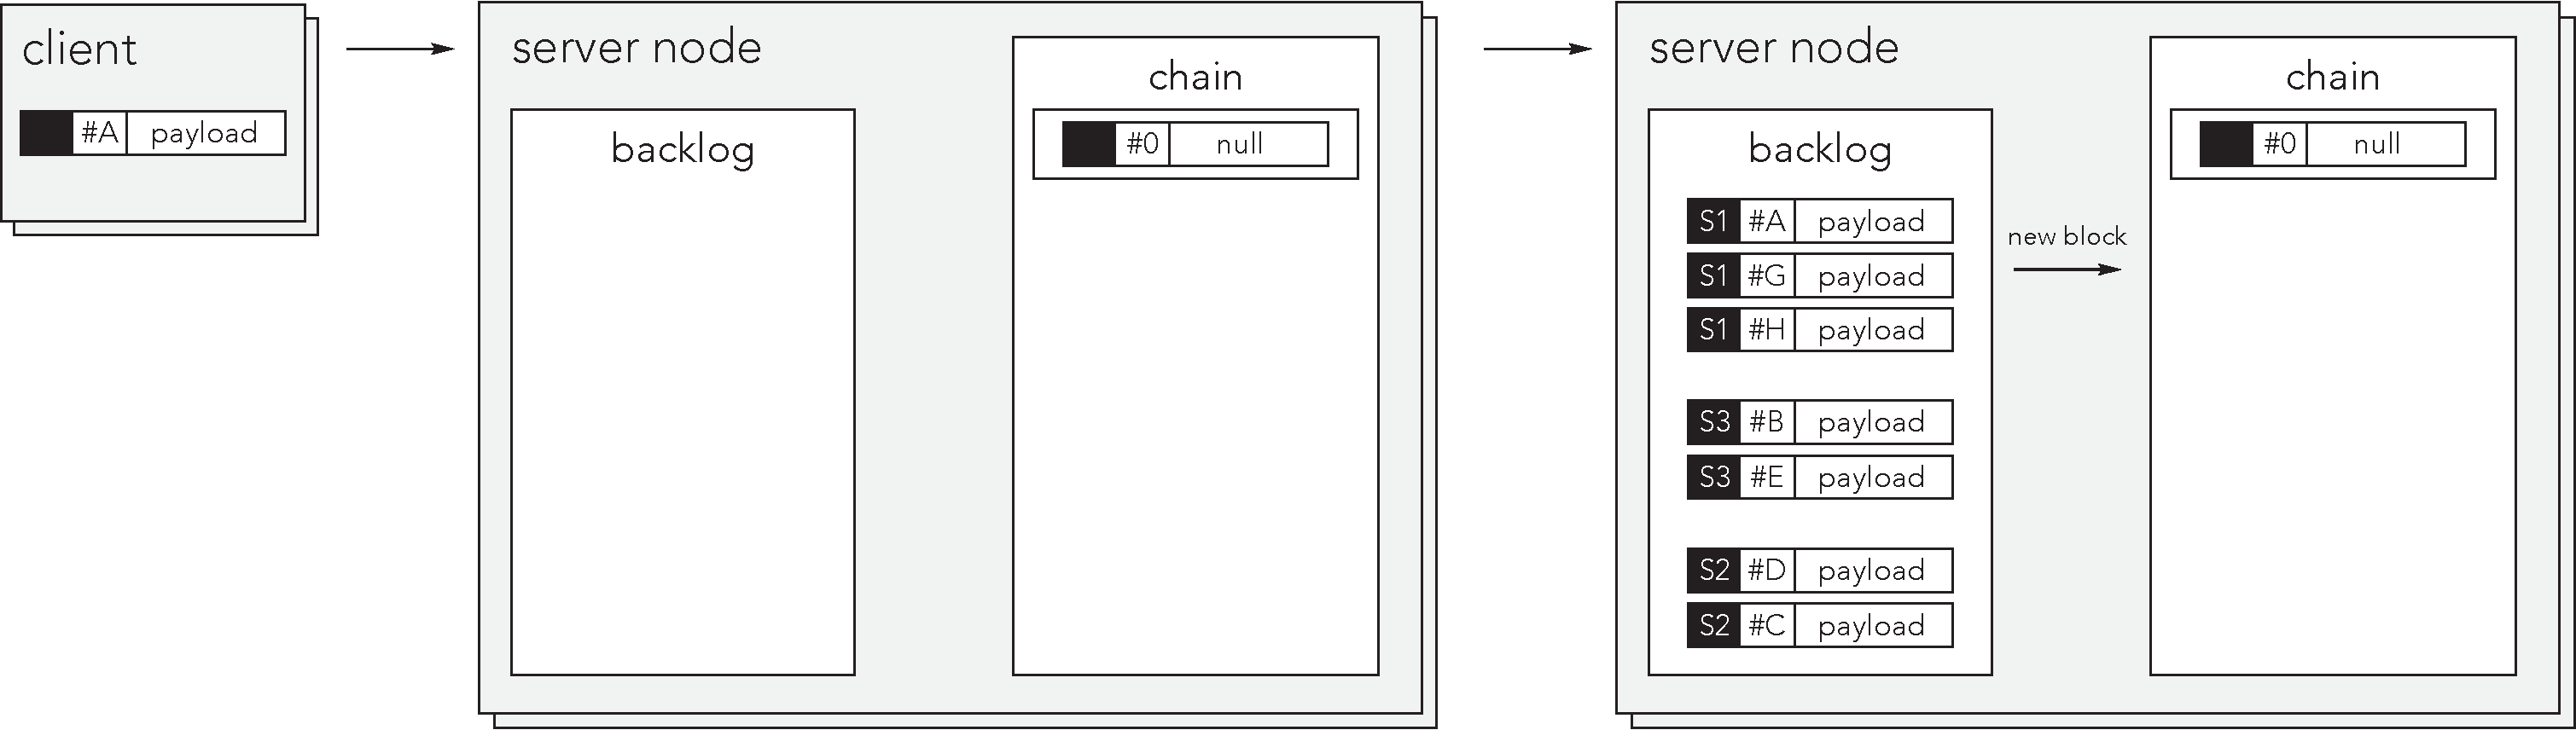
\includegraphics[width=\textwidth]{figure_4.pdf}
  \caption{\textit{Left:} BigchainDB’s backlog $\mathbf{S}$ and chain $\mathbf{C}$ start empty.
  \textit{Right:} Clients have inserted transactions into backlog $\mathbf{S}$ and assigned to nodes 1, 3, and 2.}
  \label{fig:bigchaindb_architecture_step1}
\end{figure}

Figure \ref{fig:bigchaindb_architecture_step1} and subsequent figures illustrate the high-level architecture where each card is a physical machine.
The client machines are on the left\footnote{In some images, we truncate the illustration of the client, for brevity.}.
Clients are connected to the BigchainDB server node(s) (voting node), shown on the right. Any client may send transactions to any BigchainDB server node.

In Figure \ref{fig:bigchaindb_architecture_step1} left, one client has a transaction with ID \textsf{$\#$A}, and a payload.
BigchainDB’s backlog $\mathbf{S}$ is empty; and the chain $\mathbf{C}$ is empty except for a genesis block with a null transaction.
Other clients also have transactions that they transmit to server nodes.

When a client submits a transaction, the receiving node assigns it to one of the federation nodes, possibly itself, and stores it in the backlog $\mathbf{S}$.
Figure \ref{fig:bigchaindb_architecture_step1} right illustrates an example state.
We see that node 1 is assigned three transactions, having IDs of \textsf{$\#$A}, \textsf{$\#$G}, and \textsf{$\#$H}.
Node 2 is assigned transactions with IDs \textsf{$\#$B} and \textsf{$\#$E}.
Node 3 is assigned to transactions, \textsf{$\#$D} and \textsf{$\#$C}. No transactions have been put onto the chain $\mathbf{C}$ yet.

\begin{figure}[!ht]
  \centering
  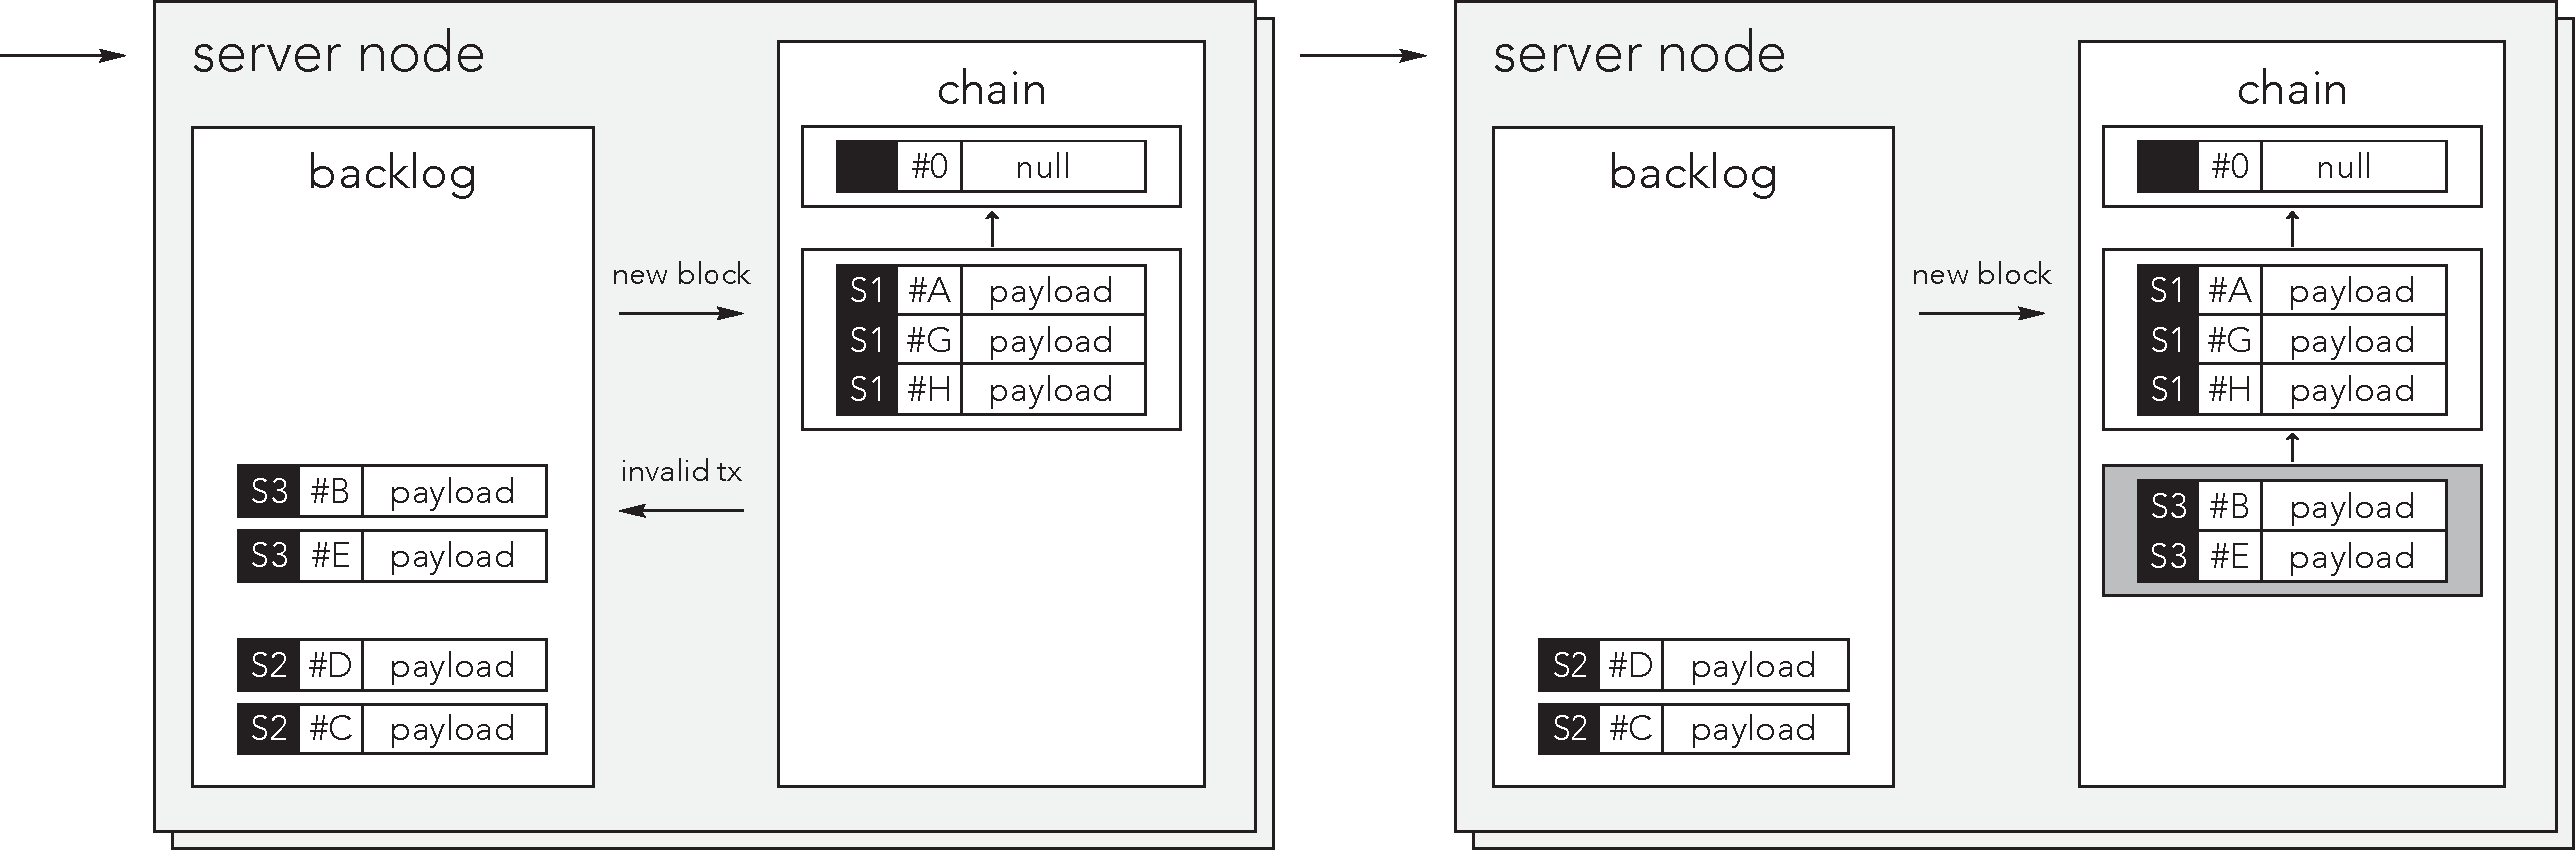
\includegraphics[width=\textwidth]{figure_5.pdf}
  \caption{\textit{Left:} Node 1 has moved its assigned transactions from backlog $\mathbf{S}$ to chain $\mathbf{C}$.
  \textit{Right:} Node 3 has processed its assigned transactions too.}
  \label{fig:bigchaindb_architecture_step2}
\end{figure}

Figure \ref{fig:bigchaindb_architecture_step2} left shows a state where Node 1 has processed all the transactions assigned to it.
It has taken the transactions \textsf{$\#$A}, \textsf{$\#$G}, and \textsf{$\#$H} from the backlog $\mathbf{S}$, created a block to hold them, then written the block onto the chain $\mathbf{C}$.
The block points to $\mathbf{C}$’s previous block.

Figure \ref{fig:bigchaindb_architecture_step2} right shows where Node 3 has processed all of its assigned transactions too, and therefore written them as a block in chain $\mathbf{C}$.

When a block is first written to $\mathbf{C}$, it starts off as \textsf{\textsf{\textit{undecided}}}.
Each server node may vote positively (for) or negatively (against) a block.
A block should only be voted positively if all previous blocks are not \textsf{\textit{undecided}}, and all transactions in the block itself are valid.
As soon as there is a majority of positive votes for a block, or a majority of negative votes, the block goes from \textsf{\textit{undecided}} to \textsf{\textit{decided\_valid}} or \textsf{\textit{decided\_invalid}}, respectively.

In this example, the block created by Node 1 gets voted on, and becomes \textsf{\textit{decided\_valid}}.
Then, the block from node 3 gets voted on, and becomes \textsf{\textit{decided\_invalid}}.
In Figure \ref{fig:bigchaindb_architecture_step2} right, we depict the distinction as a clear background for \textsf{\textit{decided\_valid}}, versus a shaded background for \textsf{\textit{decided\_invalid}}.)

\begin{figure}[!ht]
  \centering
  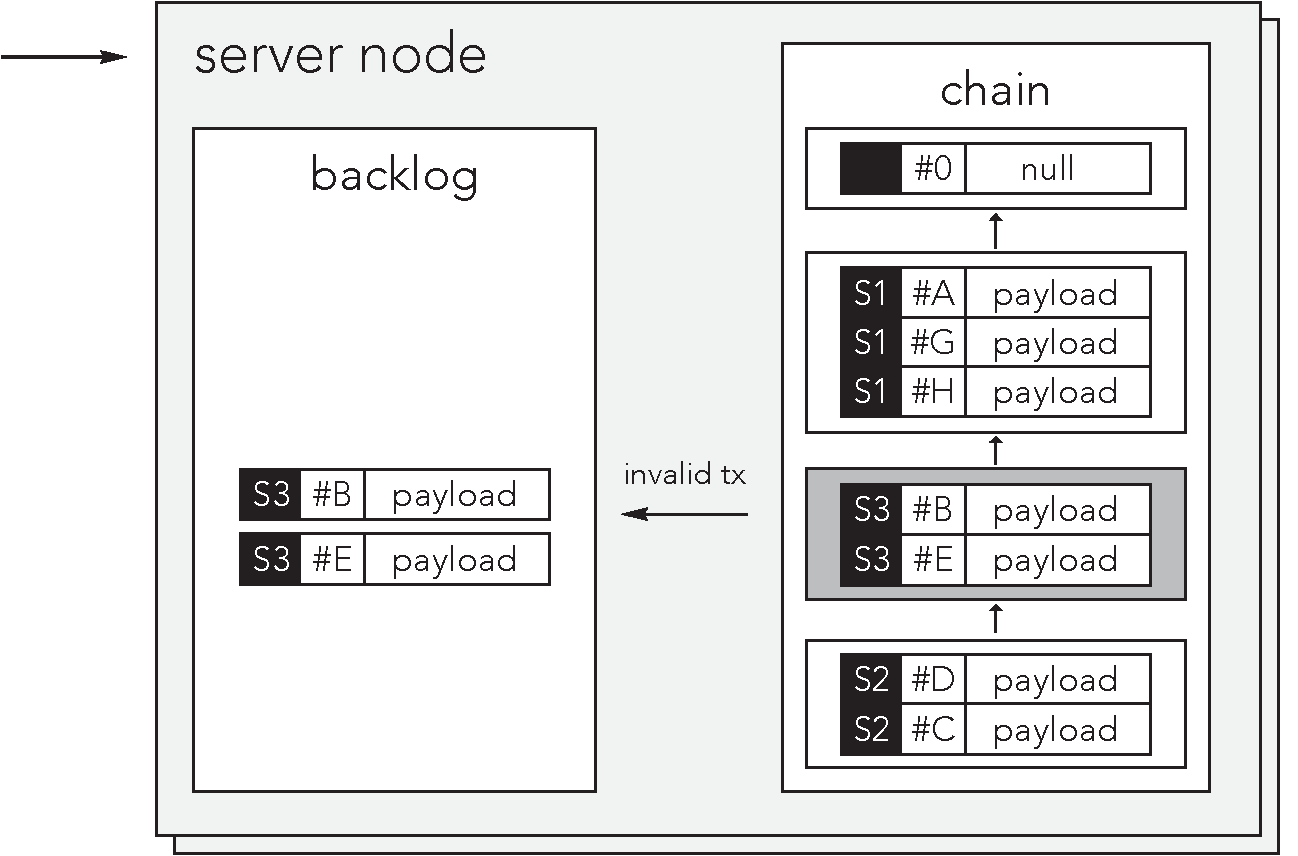
\includegraphics[width=0.5\textwidth]{figure_6.pdf}
  \caption{Transactions from an invalid block (on right, shaded) get re-inserted into backlog $\mathbf{S}$ for re-consideration.}
  \label{fig:bigchaindb_architecture_step3}
\end{figure}

While the overall block was considered invalid, some of the transactions in the invalid block may have actually been valid, and so BigchainDB gives them another chance.
Figure \ref{fig:bigchaindb_architecture_step3} illustrates how: transactions \textsf{$\#$B} and \textsf{$\#$E} get re-inserted into backlog $\mathbf{S}$ for new consideration.
Figure \ref{fig:bigchaindb_architecture_step3} also shows how BigchainDB approaches storage of invalid blocks.
There’s a block in the chain $\mathbf{C}$ that is invalid.
However, BigchainDB doesn’t remove the block; there’s no need, as the block is already marked invalid, disk space is not a problem, and it’s faster and simpler to keep all blocks there.
Similarly, voting doesn’t stop after a block becomes decided, because it’s faster for each node to simply vote than the extra step to check whether voting is necessary.

\begin{figure}[!ht]
  \centering
  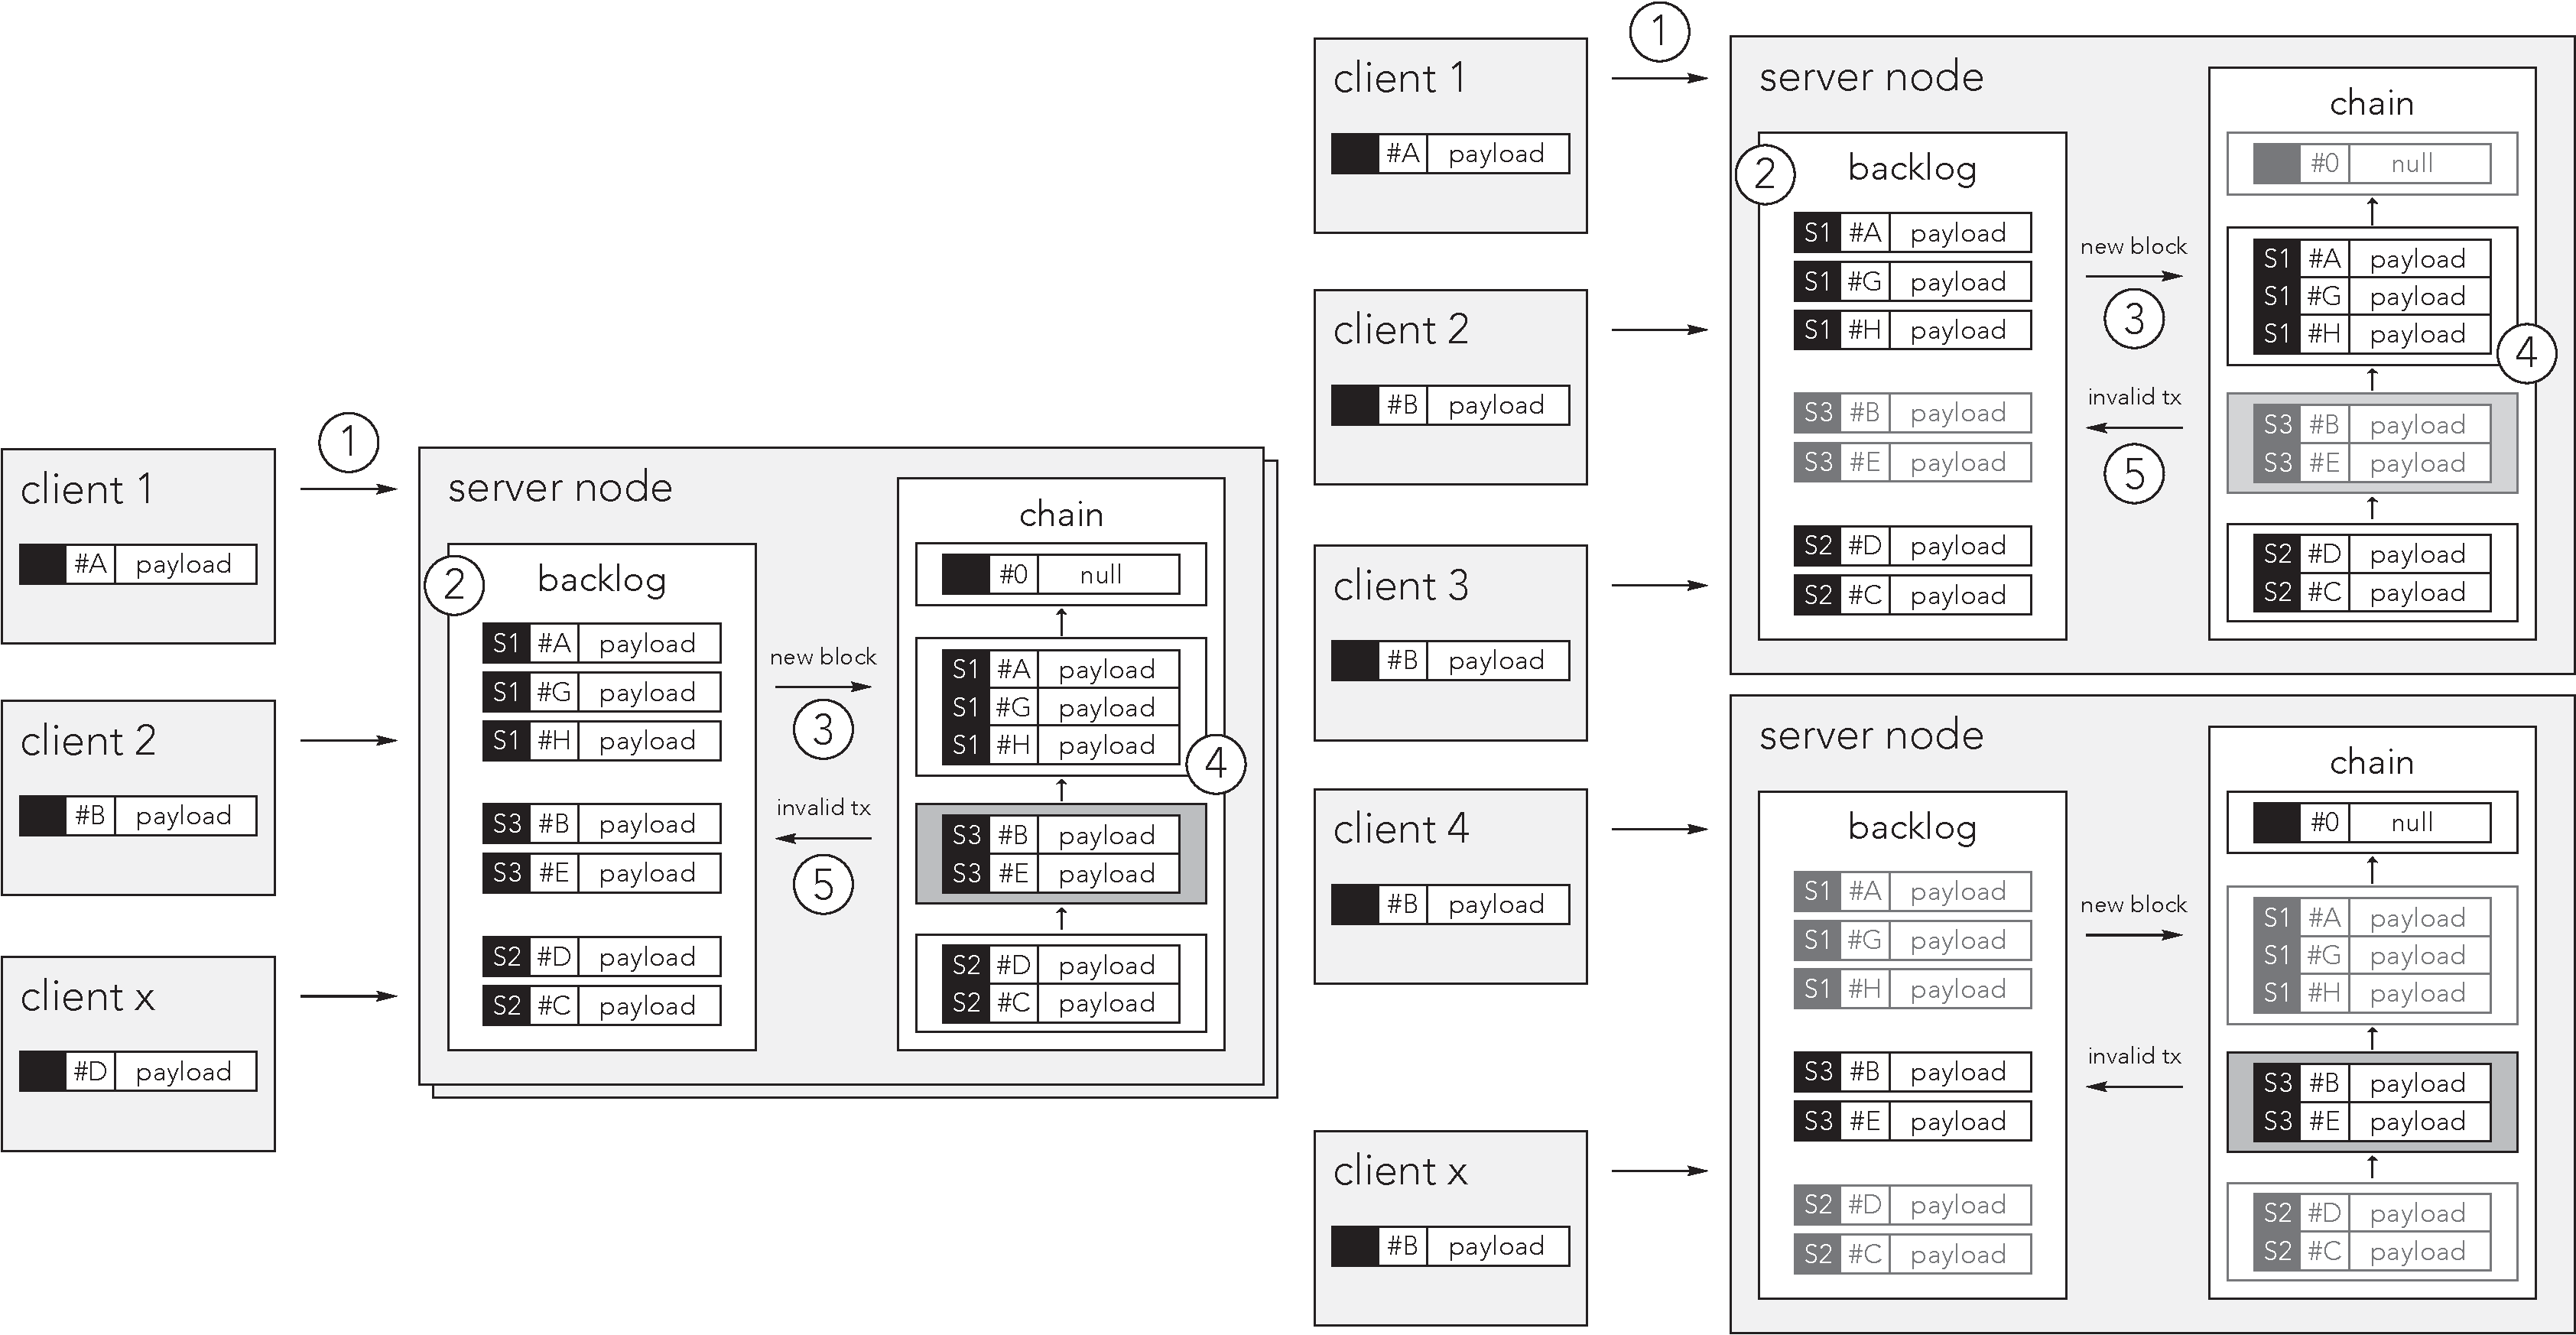
\includegraphics[width=\textwidth]{figure_7.pdf}
  \caption{\textit{Left:} More than one client may talk to a given node.
  \textit{Right:} there are multiple nodes. Typically, a client connects to just one node (an arbitrarily picked one).}
  \label{fig:bigchaindb_architecture_sharding}
\end{figure}

Figure \ref{fig:bigchaindb_architecture_sharding} emphasizes how multiple machines are configured.
Figure \ref{fig:bigchaindb_architecture_sharding} left shows that more than one client may talk to a given node.
Figure \ref{fig:bigchaindb_architecture_sharding} right shows that there is more than one node, though each node has a view into the backlog $\mathbf{S}$ and the chain $\mathbf{C}$.


\subsection{Models}\label{subsec:bigchaindb:models}
\subsubsection{Transaction Model}
A transaction is an operation between the $\mathtt{current\_owner}$ and the $\mathtt{new\_owner}$ over the digital content described by hash.
For example, it could be a transfer of ownership of the digital content hash.
A transaction has the following attributes:

\begin{lstlisting}[style=json]
{
  "id": "<sha3 hash>",
  "transaction": {
    "current owner": "<pub-key>",
    "new owner": "<pub-key>",
    "input": "<sha3 hash>",
    "operation": "<string>",
    "timestamp": "<rethinkdb timestamp>", 
    "data": {
      "hash": "<sha3 hash>",
      ...
    } 
  },
  "signature": "<ECDSA signature of the transaction>"
}
\end{lstlisting}

Attribute details are:
\begin{itemize}
 \item $\mathtt{id}$: SHA3 hash of the transaction and the DB primary key. By using the hash of the transaction of the primary key we eliminate the problem of duplicated transactions, if for some reason two nodes decide to create the same transaction 
 \item $\mathtt{current\_owner}$: Public key of the current owner of the digital content with hash $\mathtt{hash}$
 \item $\mathtt{new\_owner}$: Public key of the new owner of the digital content with hash $\mathtt{hash}$
 \item $\mathtt{input}$: SHA3 hash of the transaction in which the content was transferred to the user (similar to input in the blockchain). This will be extended to allow multiple inputs per transaction. 
 \item $\mathtt{operation}$: String representation of the operation being performed (REGISTER, TRANSFER, \ldots) to define how the transactions should be validated 
 \item $\mathtt{timestamp}$: Time of creation of the transaction in UTC 
 \item $\mathtt{data}$: JSON object describing the asset (digital content). It contains at least the field \texttt{hash}, which is a SHA3 hash of the digital content. 
 \item $\mathtt{signature}$: ECDSA signature of the transaction with the $\mathtt{current\_owner}$ private key
\end{itemize}

\subsubsection{Block Model}
A block contains a group of transactions and includes the hash of the hash of the previous block to build the chain, as follows:

\begin{lstlisting}[style=json]
{
  "id": "<sha3 hash of the list of transactions + timestamp + nodes_pubkeys>",
  "block": {
    "timestamp": "<RethinkDB timestamp>",
    "transactions": ["<list of transactions>"], 
    "node_pubkey": "<public key of the node creating the block>", 
    "voters": ["<list of federation nodes pulic keys>"]
  },
  "signature": "<signature of the block>",
  "votes": []
}
\end{lstlisting}

\begin{itemize}
  \item $\mathtt{id}$: SHA3 hash of the current block. This is also a DB primary key, to ensure we that all blocks are unique. 
  \item $\mathtt{block}$: The actual block
    \begin{itemize}
      \item $\mathtt{timestamp}$: Timestamp when the block was created 
      \item $\mathtt{transactions}$: List of transactions to be included in the block 
      \item $\mathtt{node\_pubkey}$: the public key of the node that created the block 
      \item $\mathtt{voters}$: list of public keys of the federation nodes. Since the size of the federation may change over time this will tell us how many nodes existed in the federation when the block was created so that in a later point in time we can check that the block received the correct number of votes.
    \end{itemize}
  \item $\mathtt{signature}$: Signature of the block by the node that created the block
  \item $\mathtt{votes}$: Initially an empty list. Nodes in the voters list will append to it has they vote on the block
\end{itemize}

\subsubsection{Vote Model}
This is the structure that each node will append to the block votes list. 

\begin{lstlisting}[style=json]
{
  "node_pubkey": "<the pubkey of the voting node>",
  "vote": {
    "voting_for_block": "<id of the block the node is voting for>",
    "previous_block": "<id of the block previous to this one>", 
    "is_block_valid": "<true|false>", 
    "invalid_reason": "<None|DOUBLE_SPEND|TRANSACTIONS_HASH_MISMATCH|NODES_PUBKEYS_MISMATCH>", 
    "timestamp": "<rethinkdb timestamp of the voting action>" 
  },
  "signature": "<ECDSA signature of vote block>" 
}
\end{lstlisting}


\subsection{Block Validity and Blockchain Pipelining}

\begin{figure}[!ht]
  \centering
  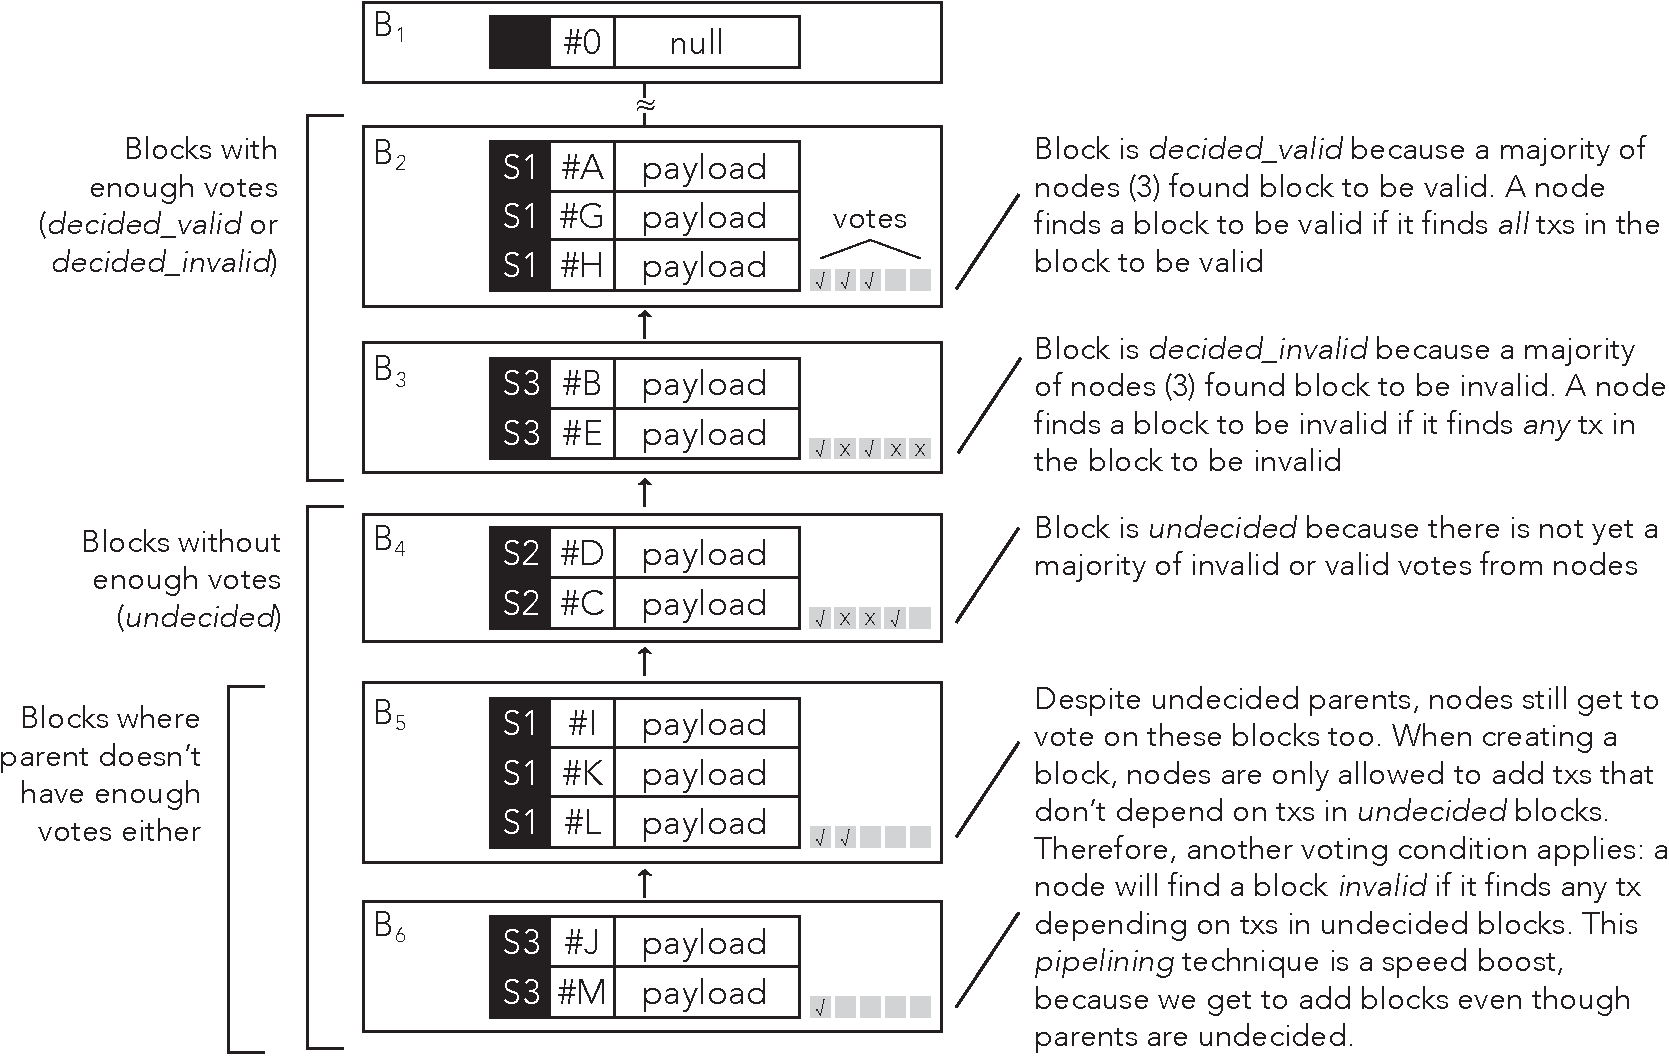
\includegraphics[width=\textwidth]{figure_8.pdf}
  \caption{Pipelining in the BigchainDB blockchain $\mathbf{C}$.
  Votes accumulate on each block.
  Blocks can continue to accumulate on the blockchain, even though their parents, grandparents, etc. may be undecided.
  The key is that when adding a new block, we can include transactions that do not depend on transactions in undecided blocks.}
  \label{fig:bigchaindb_chain_pipelining}
\end{figure}

Figure \ref{fig:bigchaindb_chain_pipelining} shows an example of a blockchain $\mathbf{C}$.
Block $\mathbf{B}_1$ is the genesis block with a null transaction.

Blocks are written in the order decided by the DB’s built-in consensus algorithm.
This means that when a signing node inserts a Block into the blockchain, it cannot provide a vote at the same time.
Only after the write is fully committed does the order become clear.

Nodes vote on blocks after order becomes clear\footnote{For example: the order of events in RethinkDB is guarantueed by the Raft consensus and does not depend on timing.}.
When a block is written, it starts off as undecided.
As soon as there is majority of positive votes for a block, or a majority of negative votes, the block goes from \textsf{\textit{undecided}} to \textsf{\textit{decided\_valid}} or \textsf{\textit{decided\_invalid}}, respectively.

Note that, unlike a typical block chain, the Block Model doesn't have a top-level link to the previous block.
Instead, it has a list of votes, and each vote has a \texttt{"previous\_block": "<id\ of\ the\ block\ previous\ to\ this\ one>"}.
If for some reason, the nodes disagree on the parent (eg. malicious nodes) on can just mark the block as invalid, return the transactions to the backlog and try again.
Chainification happens at \textit{voting} time, not at the time the block was first written to the DB.

Block $\mathbf{B}_2$ has received three votes of five possible.
In this example, all three votes are positive.
Since the majority of nodes voted that the block is \textsf{\textit{valid}}, the block is considered \textsf{\textit{decided\_valid}}.

Block $\mathbf{B}_3$ has received five votes of five possible.
There was a positive vote, then negative, then positive, then two more negative votes.
Since the majority of nodes voted that the block is \textsf{\textit{invalid}}, the block is considered \textsf{\textit{decided\_invalid}}.
This block can stay in the chain because all the votes show that it is invalid.
It will be ignored when validating future transactions.
By keeping the block in place, we can quickly progress the chain to child blocks.

Block $\mathbf{B}_4$ is \textsf{\textit{undecided}} because it does not yet have a majority of invalid or valid votes from nodes.
Voting on $\mathbf{B}_4$ continues.

It is crucial that despite $\mathbf{B}_4$ being \textsf{\textit{undecided}}, it still has a child block $\mathbf{B}_5$.
This is possible because the DB’s built-in consensus algorithm determines the order of the blocks, and we have logically separated writing blocks from voting.
“Forking” is not a risk as it is not even in the vocabulary of the DB, let alone supported in code.
The reason is that every node is working on the same blockchain (instead of every node working on their own replica of the blockchain which may be different from the other nodes) and every node communicates through the database which is basically and open broadcast channel (instead of on communicating individually with each node).
Because of this, any node can try to add a block, but only one becomes the child to $\mathbf{B}_4$; the rest follow according to the built-in consensus algorithm.
It is a single railroad track where the location of the next plank is based on previous planks.
We do not have to stop at adding a single plank after an undecided block—we can keep aggressively laying track, such as block $\mathbf{B}_6$ in the figure.

When there are undecided parent blocks, we need to do one more thing to prevent double-spending: any transaction put into a new block must not depend on transactions in an undecided block.
For example, inputs of a new transaction must not be in inputs of any undecided blocks.
This is enforced in two ways: when creating new blocks on undecided blocks, such double-spend transactions are not allowed, and when voting, any block containing such transactions is voted invalid.

We call this “blockchain pipelining” because this behavior is reminiscent of pipelining in microprocessors.
There, the microprocessor starts executing several possible instructions at once.
Once the microprocessor has worked out the proper order for the instructions, it collates the results as output and ignores useless results.
As with microprocessor pipelining, blockchain pipelining gives significant speed benefits.

\subsection{BigchainDB Consensus Algorithm (BCA)}

The BigChainDB Consensus Algorithm (BCA) is a state machine that runs on each “signing” node (server).
This section outlines the BCA using Python-like pseudocode.\footnote{The actual code will be open source, so if you’re curious about implementation details, you can read that.}

\subsubsection{Main Loop}

Before starting the $\mathtt{mainLoop()}$ on each signing node, the databases $\mathbf{S}$ and $\mathbf{C}$ must be created and initialized.
One of the initialization steps is to write a genesis block to $\mathbf{C}$.

Listing \ref{lst:bca} has high-level pseudocode for the BCA.
It shows the $\mathtt{mainLoop()}$ running on signing node $\mathbf{k}$.
Every signing node runs the same $\mathtt{mainLoop()}$.

Line $\mathtt{4}$ emphasizes that there is equal access by all the nodes to the databases $\mathbf{S}$ and $\mathbf{C}$. 
The BCA operates by moving data from transaction set $\mathbf{S}$ to blockchain $\mathbf{C}$, and occasionally in the other direction as well.

\begin{minipage}{\linewidth}
  \begin{lstlisting}[caption={BigchainDB Consensus Algorithm. This algorithm runs on every signing node.}, label={lst:bca}, style=python]
  def mainLoop(): # Pseudocode for signing node k 
    # Assume S and C exist and are initialized,
    # and C contains a genesis block. 
    global S, C # tx set and blockchain globally visible
    while True: 
      S = assignTransactions(S, k) 
      Sk, C = addBlock(Sk, C, k) 
      C = voteOnBlocks(C, k)
  \end{lstlisting}
\end{minipage}

Line $\mathtt{5}$ is the start of the main loop. All remaining pseudocode is part of this loop, which runs continuously until the node is shut down.

Line $\mathtt{6}$ accepts transactions to into $\mathbf{S}$ and assigns them to nodes, line $\mathtt{7}$ moves unordered transactions from $\mathbf{S}$ into ordered, grouped-by-block transactions in $\mathbf{C}$, and line $\mathtt{8}$ is where the node votes on undecided blocks.

\begin{minipage}{\linewidth}
  \begin{lstlisting}[caption={Parallel version of BigchainDB Consensus Algorithm.}, label={lst:bca_parallel}, style=python]
  def mainLoopParallel():
    start => 1 assignTransactionLoop() processes 
    start => 1 addBlockLoop() processes 
    start => 1 voteLoop() processes
    
  def assignTransactionLoop():
    while True:
      S = assignTransactions(S, k)
  
  def addBlockLoop():
    while True:
      Sk, C = addBlock(Sk, C, k)
  
  def voteLoop():
    while True:
      C = voteOnBlocks(C, k)
  \end{lstlisting}
\end{minipage}

The pseudocode of Listing \ref{lst:bca} is written as if there is a single process.
But each major step can actually be a separate, independent process.
In fact, there can be multiple processes doing each step; this helps performance tremendously.
Listing \ref{lst:bca_parallel} shows the pseudocode.

\subsubsection{Assigning Transactions}

\medskip
\noindent Listing \ref{lst:bca_tx_routines} algorithms are for assigning transactions, as follows:

Listing \ref{lst:bca_tx_routines} $\mathtt{assignTransactions()}$ is the main routine that groups the two major steps: accepting and assigning incoming transactions (line $\mathtt{2}$), and reassigning old transactions (line $\mathtt{3}$).

Listing \ref{lst:bca_tx_routines} $\mathtt{assignNewTransactions()}$ accepts incoming transactions from clients of the BigchainDB and assigns transactions to nodes.
We assign transactions to a node rather than allowing nodes to grab transactions, because assignment greatly reduces double-spend detections in the block chain building side, and therefore helps throughput.
We considered assigning nodes deterministically, for example based on the hash of the transaction.
However, that would be problematic if a malicious node repeatedly inserted a bad transaction into $\mathbf{C}$, then when it got kicked back to $\mathbf{S}$, the malicious node got the same transaction again.
Instead, we assign the node randomly with equal probability to each node, except the current node $\mathbf{k}$ in order to avoid a duplicate vote.

In the algorithm, line $\mathtt{7}$ accepts transactions and loops through them; line $\mathtt{8}$ chooses which node, with uniform probability; line $\mathtt{9}$ records the assign time (see the next algorithm for why); and line $\mathtt{10}$ actually assigns the transaction to the chosen node.

\begin{minipage}{\linewidth}
  \begin{lstlisting}[caption={Routines for accepting and assigning transactions.}, label={lst:bca_tx_routines}, style=python, mathescape=true]
  def assignTransactions(S, k):
    S = assignNewTransactions(S, k) 
    S = reassignOldTransactions(S, k) 
    return S 
    
  def assignNewTransactions(S, k): 
    for each new tx, t from outside: 
      i $\sim$ U({0, 1, $\dots$, k-1, k+1, $\dots$, N-1}) # Stochastic. Any node but k avoids duplicate vote. 
      t.assign_time = time() 
      Si = Si $\cup$ t 
      return S 
    
  def reassignOldTransactions(S, k): 
    for Sj in {S1, S2, $\dots$}: 
      for each tx, t, in Sj: 
        if (time() - t.assign_time) > old_age_thr:
          i $\sim$ findex(t) # deterministic function of t
          t.assign_time = time()
          Si = Si $\cup$ t
          Sj = Sj - t
    return S
  \end{lstlisting}
\end{minipage}

Listing \ref{lst:bca_tx_routines} $\mathtt{reassignOldTransactions()}$ re-assigns transactions that are too old.
Transactions can get old if a node goes down, is running slowly, is acting maliciously, or is not performing its duties more generally.
This routine ensures transactions assigned to a node are not dropped, by re-assigning old transactions to a different node.
It loops through all assigned transactions (lines $\mathtt{14}$-$\mathtt{15}$), and if the transaction’s previous assignment is too old (line $\mathtt{16}$) it chooses a new node (line $\mathtt{17}$), sets a new assign time (line $\mathtt{18}$), and moves the transaction assignment from the old node (node \textbf{j}) to the new node (node \textbf{i}).
For this routine to work, it also needs the unassigned-transactions to have an assign time, which is done in $\mathtt{assignNewTransactions()}$ (line $\mathtt{9}$)).

In line $\mathtt{17}$, the node assignment is not random, but instead deterministic as a function of the transaction.
This is so nodes do not inadvertently fight over which node gets the transaction $\mathbf{t}$.
An example deterministic function $f_{\mathtt{index}}(\mathbf{t})$ is $\mathtt{mod}(\mathtt{hash}(\mathbf{t}))$—hash the transaction then modify it by the number of nodes.

\subsubsection{Adding and Voting on Blocks}

\medskip
Listing \ref{lst:bca_block_add} $\mathtt{addBlock()}$ creates and adds a (non-genesis) block to $\mathbf{C}$, and ends with a set of transactions to postpone

\begin{minipage}{\linewidth}
  \begin{lstlisting}[caption={Routine for adding normal blocks.}, label={lst:bca_block_add}, style=python, mathescape=true]
  def addBlock(Sk, C, k):
    $\mathtt{T}_{\mathtt{postpone}}$ = {}
    $\mathtt{B}_{\mathtt{new}}$ = $\varnothing$
    $\mathtt{B}_{\mathtt{tail}}$ = most recent block in C
    $\mathtt{T}_{\mathtt{new}}$ = []
    for t in Sk:
      if dependsOnUndecidedBlock(t, $\mathtt{B}_{\mathtt{tail}}$):
        $\mathtt{T}_{\mathtt{postpone}}$ = $\mathtt{T}_{\mathtt{postpone}}$ $\cup$ t
      elif transactionValid(t, $\mathtt{B}_{\mathtt{tail}}$):
        $\mathtt{T}_{\mathtt{new}}$.append(t)
    id = sha3 hash of {$\mathtt{T}_{\mathtt{new}}$, other data wrt Sec. 5.5}
    votes = []
    $\mathtt{B}_{\mathtt{new}}$ = Block(id, $\mathtt{T}_{\mathtt{new}}$, votes, other data wrt Sec. 5.5)
    add $\mathtt{B}_{\mathtt{new}}$ to C # C’s consensus algorithm will determine order
    Sk = $\varnothing$
    Sk = Sk $\cup$ $\mathtt{T}_{\mathtt{postpone}}$
    return Sk, C
  \end{lstlisting}
\end{minipage}

Lines $\mathtt{2-3}$ initialize the routine’s main variables – the block to add $\mathbf{B}_{\mathtt{new}}$, and the transactions to postpone adding until later $\mathbf{T}_{\mathtt{postpone}}$.

Lines $\mathtt{4-17}$ creates a block and adds it to $\mathbf{C}$, in an order determined by $\mathbf{C}$’s consensus algorithm.
Line $\mathtt{4}$ updates its pointer $\mathbf{B}_{\mathtt{tail}}$ to the most recent block in $\mathbf{C}$.
It is important to grab $\mathbf{B}_{\mathtt{tail}}$ here rather than computing it on-the-fly, in case new blocks are added while the rest of the routine is running.
Line $\mathtt{5}$ initializes the ordered list of transactions to be added to the block, and lines $\mathtt{7-10}$ add them one at a time.
If a transaction $\mathbf{t}$ depends on an \textsf{\textit{undecided}} block (risking double-spend) it will be postponed to another block by being added to $\mathbf{T}_{\mathtt{postpone}}$ (lines $\mathtt{7-8}$).
Otherwise, if it is considered valid, then it is added to $\mathbf{T}_{\mathtt{new}}$ (lines $\mathtt{9-10}$).
Otherwise, it will be discarded. Lines $\mathtt{11-14}$ create the block and add it to $\mathbf{C}$.

Listing \ref{lst:bca_block_add} lines $\mathtt{15-16}$ occur once the block has been successfully added. With new transactions now in $\mathbf{C}$, those transactions can be removed from $\mathbf{S}$, as line $\mathtt{15}$ does by clearing $\mathbf{S}_k$.
Line $\mathtt{16}$ reconciles by adding back any postponed transactions, for example any transactions that risked being double-spends due to being added after an \textsf{\textit{undecided}} block.

\begin{minipage}{\linewidth}
  \begin{lstlisting}[caption={Routine for voting on blocks.}, label={lst:bca_block_vote}, style=python, mathescape=true]
  def voteOnBlocks(C, k): 
    B = oldest block in C that node k hasnt voted on
    while B: 
      vote = transactionsValid(B)
      B.V[k] = vote
      if B is decided and invalid: copy B’s txs back into S 
      B = (child block of B) or $\varnothing$
    return C
  \end{lstlisting}
\end{minipage}

\noindent Listing \ref{lst:bca_block_vote}: Routine for voting on blocks $\mathtt{voteOnBlocks()}$ is the routine for node $\mathbf{k}$ to vote on blocks that it hasn’t yet voted on.

Note that a node actually votes on blocks that may have already been decided, because it’s faster to vote than to first query whether the block is decided.
Lines $\mathtt{3-8}$ iterate from the oldest block that node $\mathbf{k}$ hasn’t voted on (found in line $\mathtt{2}$) to the newest block (when temporary variable goes to $\varnothing$ in line $\mathtt{7}$).
For each block, line $\mathtt{4}$ computes a Boolean of whether all transactions in the block $\mathbf{B}$ are valid, and line $\mathtt{5}$ stores that in $\mathbf{B}$’s votes variable $\mathbf{B.V}$, signed by node $\mathbf{k}$.
Line $\mathtt{6}$ gives potentially valid transactions another chance.

\subsubsection{Transaction Validity}

\begin{minipage}{\linewidth}
  \begin{lstlisting}[caption={Routines for transaction validity.}, label={lst:bca_tx_valid}, style=python, mathescape=true]
  def transactionsValid(T, Bi):
    # are all txs valid?
    for t in T:
      if not transactionValid(t, Bi):
        return False
      return True
  
  def transactionValid(t, Bi):
    # Is tx valid in all blocks up to and including Bi? 
    # (Ignore Bi+1, Bi+2, $\dots$) 
    if t is ill-formed, commits double-spend, etc. 
      return False
    if dependsOnUndecidedBlock(t, Bi)
      return False
    return True
    
  def dependsOnUndecidedBlock(t, Bi):
    # returns True if any of t’s inputs are in a block 
    # that is not voted enough (enough x's or $\surd$'s) 
    # in [B0, B1, $\dots$ , Bi]. Ignores [Bi+1, Bi+2, $\dots$]
  \end{lstlisting}
\end{minipage}

\medskip
\noindent Listing \ref{lst:bca_tx_valid} holds the routines for measuring validity of transactions.

\medskip
\noindent Listing \ref{lst:bca_tx_valid} $\mathtt{transactionsValid()}$ is the top-level routine to simply loop through all the transactions supplied in the transaction list $\mathbf{T}$ (lines $\mathtt{3-6}$), and if any transaction is found to be invalid (line $\mathtt{4}$) the routine returns False.

\medskip
\noindent Listing \ref{lst:bca_tx_valid} $\mathtt{transactionValid()}$ measures whether a transaction is valid, based on traditional blockchain validity measures (ill-formed, double-spend, etc.) in lines $\mathtt{11-12}$ and also based on whether it depends on an undecided block (lines $\mathtt{13-14}$).

\medskip
\noindent Listing \ref{lst:bca_tx_valid} $\mathtt{dependsOnUndecidedBlock()}$ clarifies what it means to depend on an undecided block.

\subsection{Consensus Algorithm Checklist}
As we were designing the BCA, we encountered some pitfalls and concerns that we subsequently resolved.

\medskip
\noindent\textbf{Client transaction order.} We must ensure that transactions sent from the same client, or at least transactions received in a particular order, are processed in that order—or at least with a bias to that order.
A typical scenario is where a client’s first transaction is to fill a value at an address, and second transaction is to spend from it.
For starters, this should not be rejected.
Better yet, it should go through the system efficiently, which means that there should (at the very least) be a bias to process the first client transaction before the second client transaction.

\medskip
\noindent\textbf{Block construction order.}
By the time we create memory space for a block at address $\alpha$, all its transactions must be in the block, so that blocks added after $\alpha$ can check to not double-spend those transactions.
This would fail if node 1 creates a block $\mathbf{B}_1$ at $\alpha_!$, then node 2 creates a block $\mathbf{B}_2$ that follows $\mathbf{B}_1$, then node 2 adds transactions to $\mathbf{B}_2$, then node 1 adds transactions to $\mathbf{B}_1$ which invalidate some of the transactions in $\mathbf{B}_2$.

\medskip
\noindent\textbf{Hashing votes.} Is there transaction malleability because votes are not hashed?
This may look like a problem, because a block’s hash can be propagated to its child block before all its votes are in.
A preliminary answer would be to have a second chain of hashes that actually includes the votes.
But the solution can be simpler than that: a single hash (without votes) is fine because the votes are digitally signed by the signing nodes, and therefore not malleable.

\medskip
\noindent\textbf{Dropping transactions.} If a node goes down, what happens to the transactions assigned to it? Do those transactions get dropped?
In our initial design, the answer was mostly no, because all transactions are stored in $\mathbf{S}$ until they have been committed to a block.
However, if a node went down or, more generally misbehaved, transactions assigned to that node might not be handled.
To address this, we added a way to re-assign transactions if the previous node assignment got stale: algorithm $\mathtt{reassignOldTransactions()}$ in Listing \ref{lst:bca_tx_routines}.

\medskip
\noindent\textbf{Denial of service.} Are there any transactions that can be repeatedly called by aggressor clients or a malicious server node, which tie up the network?
To our knowledge, this is not an issue any more than with a traditional web service.

\medskip
\noindent\textbf{Database built-in communication vulnerability.} The nodes communicate using the big data DB’s own built-in consensus algorithm like Paxos to tolerate benign failures. 
Is this a vulnerability? The answer is that a majority of the network would need to be affected for it to have any major consequences.

\medskip
\noindent\textbf{Double spends.} Are there any ways to double-spend? 
This is a useful question to keep asking at all stages of development. 
In this regard BigchainDB does exactly the same as the bitcoin network. All past transactions are checked to make sure that input was not already spent.

\medskip
\noindent\textbf{Malicious behavior.} Questions: How does BigchainDB detect that a node has bad (Byzantine) behavior? 
Does it discourage bad behavior? How? 
Answers: Overall, it’s a simpler problem because of the federation model. 
Bad behavior can be detected when a node’s vote on a block is different than the majority. 
There are many possible ways to discourage bad behavior, from manual punishment decided by the federation, to needing to post a security deposit (bond) and automatically losing it upon bad behavior. 

\medskip
\noindent\textbf{Admin becoming god.} Does the system administrator have any powers that allow them to play “god”, and thus constitute a single point of failure? 
We were careful to limit the power of the system administrator to even less than a voting node. 
So to our knowledge, the system administrator cannot play god because all write transactions (including updating software) need to be voted on by the federation. 

\medskip
\noindent\textbf{Offline nodes.} Q: What happens if a voting node goes offline? If many go offline? 
A: One or a few offline is fine, as quorum (the number of nodes needed to approve a transaction) is still met. 
Typically, quorum is a majority of nodes. Split votes or many offline nodes could leave a block in an undecided state. 
This implies that transactions that depend on the undecided block (i.e. transactions who’s input is an output of a transaction that is in an undecided block) will remain in the backlog until enough voting nodes are back online to resolve the split vote or undecided state. 
Alternative measures could be to leave a block in an undecided state for a limited amount of time. 
Once the time threshold is reached, the block is automatically rejected and the transactions return to the backlog. 
Also, pending split votes may be resolved as being rejected using a more pessimistic voting strategy. 

\medskip
\noindent\textbf{Hash at block vs transaction level.} Q: Why do we chain together blocks, rather than chaining together transactions, which is simpler? 
A: There are two reasons. 
First, with distributed data stores, there is no guarantees in the order in which transactions will be committed to the DB. 
Without knowing what is previous transactions to be committed to the DB, we cannot include its hash in the current transaction to build the chain. 
To solve this problem we decided to use blocks and create the chain with the blocks. 
Second, it is more efficient to group transaction into batches for the surrounding logic – the cost gets amortized over the whole block. 
For example, only one hash for every block rather than every transaction.


\subsection{Transaction Validity, Incentivization, and Native Assets}
Each BigchainDB transaction has inputs and outputs.
As with Bitcoin, the key measure of transaction validity is whether the inputs have sufficient funds to cover the outputs: “you can only spend what you have.”
Validity is measured by voting nodes.

Recall that BigchainDB consensus is federation-based.
A node gets to vote on a transaction based on whether it has been given a voting node role.
Contrast this to a POW model, where the probability of a node voting is proportional its hash power, which assuming all miners have state-of-the-art hardware is equivalent to electricity spent; or to POS where probability of a node voting is proportional to how much money it has.

Traditionally, blockchains have held two types of assets. 
“Native assets” like Bitcoins or Ether are built into the core protocol. 
The consensus uses these assets to measure transaction validity and to reward voting by native-asset transaction fees and mining rewards. 
Second are non-native “overlay assets” in overlay protocols sitting above the core protocol (e.g. SPOOL \cite{dejonghe_spool}).
However, this traditional approach to native assets and reward has weaknesses:

\begin{itemize}
 \item \textbf{Overlay Asset Double-Spend.} Traditional blockchains’ consensus models do not account for overlay assets. There is nothing at the core protocol level to prevent a double-spend of an overlay asset.
 \item \textbf{Native Asset Friction to Network Participation.} Traditional blockchain voting nodes need to get paid in the native asset, so any new participants in the network must acquire the native asset, typically on an exchange, before being able to conduct a transaction. Acquiring the native asset is especially difficult on newer blockchains with native assets that are not yet available on many exchanges. This is a high barrier to entry when compared to traditional web services, where any new participant can conduct a transaction by paying in a standard currency like U.S. dollars with a standard payment method like a credit card.
\end{itemize}

BigchainDB overcomes these issues as follows (and as shown in Table \ref{tab:bigchain_comparison_assets}):
\begin{itemize}
 \item \textbf{Native consensus voting on every asset.} Every transaction keeps track of which asset it is operating on, chaining back to the transaction that issued the asset. Every asset is “native” in the sense that it’s used to measure transaction validity. This overcomes the issue of “asset overlay double-spend.”
 \item \textbf{Low friction to network participation.} Like a traditional web service, the network operator sets the terms on how to join the network and conduct transactions—but in this case the network operator is the collective will of the voting nodes. The voting nodes also determine how users pay for transactions.
\end{itemize}

\begin{table}[h]
  \caption{Native Assets Validity \& Incentivization}
  \footnotesize
  \makebox[\textwidth][c]{
  \centering
  \setlength\extrarowheight{3pt}
  \begin{tabular}{ | m{\dimexpr 0.3\linewidth-2\tabcolsep} |
	  M{\dimexpr 0.175\linewidth-2\tabcolsep} |
	  M{\dimexpr 0.175\linewidth-2\tabcolsep} |
	  M{\dimexpr 0.175\linewidth-2\tabcolsep} |
	  M{\dimexpr 0.175\linewidth-2\tabcolsep} |} \Xhline{4\arrayrulewidth}\rowcolor{black}
  		                    & \multicolumn{2}{|c|}{\color{white} Traditional Blockchain} & \multicolumn{2}{|c|}{\color{white} BigchainDB} \\\Xhline{4\arrayrulewidth}\rowcolor{backcolour}
  		                    & Native Asset & Overlay Assets & Native Asset & Overlay Assets \\\Xhline{2\arrayrulewidth}
  Asset Types 			    & Y (one)	   & Y (multiple)   & Y (multiple) & N          \\\hline
  Validated by Blockchain Consensus & Y 	   & N              & Y            & N/A        \\\hline
  Incentivization Via               & \multicolumn{2}{|M{\dimexpr 0.35\linewidth-2\tabcolsep}|}{Native Asset \makebox{(e.g. Mining Reward)}} & \multicolumn{2}{M{\dimexpr 0.35\linewidth-2\tabcolsep}|}{External Fees \makebox{(e.g. Transactions, Storage)}} \\\hline
  Payment for Transactions          & \multicolumn{2}{|M{\dimexpr 0.35\linewidth-2\tabcolsep}|}{Obtain Native Assets \makebox{(e.g. Via an Exchange)}} & \multicolumn{2}{M{\dimexpr 0.35\linewidth-2\tabcolsep}|}{Fiat Currency \makebox{(e.g. Traditional channels)}} \\\hline
  \Xhline{4\arrayrulewidth}
  \end{tabular}
  }
  \label{tab:bigchain_comparison_assets}
\end{table}

\subsection{Incentivization \& Security}
In POW and POS blockchains, the network, incentive model, and security of the network are inextricably linked. Security is intrinsic to the system.
But as discussed in section \ref{sec:background} and appendix \ref{appendix:blockchain_scalability}, both POW and POS have scalability challenges.
Though it’s a double-edged sword: when incentives are intrinsic to the system too, there is motivation to game the system.
An example is the emergence of mining pools to benefit the most from Bitcoin’s built-in incentive (mining rewards).

In a federation like BigchainDB, the security of each node and aggregate security over the entire network are extrinsic.
This means the rules for confidentiality, availability, and integrity are outside the core network design \cite{gault2015cia_secret}.
For instance, if all nodes have weak rules for security, the network will be breached.
By contrast, if a minimum fraction of the network nodes have reasonable security standards, the network as a whole can withstand attacks.
Extrinsic incentives can have benefits: in a private deployment, the network participants are motivated simply by the benefits of being part of the network (e.g. lower costs, lower fraud, new functionality).
Extrinsic incentives can work in a public deployment too, for similar reasons: the voting nodes may have their own reasons for an open, public database to survive, for example a mandate as a nonprofit, and this makes the interests aligned (see also section \ref{subsec:permissioning_public}).